\documentclass{ximera}
 
%% You can put user macros here
%% However, you cannot make new environments

\listfiles

\graphicspath{{./}{firstExample/}{secondExample/}}

\usepackage{tikz}
\usepackage{tkz-euclide}
\usepackage{tikz-3dplot}
\usepackage{tikz-cd}
\usetikzlibrary{shapes.geometric}
\usetikzlibrary{arrows}
\usetikzlibrary{decorations.pathmorphing,patterns}
\usetkzobj{all}
\pgfplotsset{compat=1.13} % prevents compile error.

\renewcommand{\vec}[1]{\mathbf{#1}}
\newcommand{\RR}{\mathbb{R}}
\newcommand{\dfn}{\textit}
\newcommand{\dotp}{\cdot}
\newcommand{\id}{\text{id}}
\newcommand\norm[1]{\left\lVert#1\right\rVert}
 
\newtheorem{general}{Generalization}
\newtheorem{initprob}{Exploration Problem}

\tikzstyle geometryDiagrams=[ultra thick,color=blue!50!black]

\usepackage{mathtools}
 
 
 
 
\title{6.2 Spring Problems II}
 
 
\begin{document}
 
\begin{abstract}
 We return to our study of harmonic motion as an application of second order linear differential equations, this time considering the cases where damping occurs.
\end{abstract}
 
\maketitle
 
\section*{Spring Problems II}
 
\subsection*{Free Vibrations With Damping}
 
In this section we consider the motion of an object in a spring--mass
system with damping. We start with unforced motion, so the equation of
motion is
\begin{equation}\label{eq:6.2.1}
my''+cy'+ky=0.
\end{equation}
Now suppose   the object is displaced from equilibrium and given an
initial velocity. Intuition suggests that if the damping force is
sufficiently weak the resulting motion will be oscillatory, as in the
undamped case considered in the previous section, while if it's
sufficiently strong the object may just move slowly toward the
equilibrium
position without ever reaching it. We'll now confirm these intuitive
ideas mathematically. The characteristic equation of \eqref{eq:6.2.1} is
$$
mr^2+cr+k=0.
$$
The roots of this equation are
\begin{equation}\label{eq:6.2.2}
r_1=\frac{-c-\sqrt{c^2-4mk}}{2m}\quad\mbox{and}\quad r_2=
\frac{-c+\sqrt{c^2-4mk}}{2m}.
\end{equation}
In \href{https://ximera.osu.edu/ode/main/constantCoefficientHomogeneousEquations/constantCoefficientHomogeneousEquations}{Trench 5.2} we saw that the form of the
solution of  \eqref{eq:6.2.1} depends upon whether $c^2-4mk$ is positive,
negative, or zero. We'll now consider these three cases.
 
\subsection*{Underdamped Motion}
 
We say the motion is \textit{underdamped} if $c<\sqrt{4mk}$. In this
case $r_1$ and $r_2$ in \eqref{eq:6.2.2} are complex conjugates, which we
write as
$$
r_1=-\frac{c}{2m}-i\omega_1\quad\mbox{and}\quad
r_2=-\frac{c}{2m}+i\omega_1,
$$
where
$$
\omega_1=\frac{\sqrt{4mk-c^2}}{2m}.
$$
The general solution of  \eqref{eq:6.2.1} in this case is
$$
y=e^{-ct/2m}(c_1\cos\omega_1 t+c_2\sin\omega_1 t).
$$
By the method used \href{https://ximera.osu.edu/ode/main/springProblemsI/springProblemsI}{Trench 6.1}
to derive the
amplitude--phase form of the displacement of an object in simple
harmonic motion, we can rewrite this equation as
\begin{equation}\label{eq:6.2.3}
y=Re^{-ct/2m}\cos(\omega_1 t-\phi),
\end{equation}
 where
$$
R=\sqrt{c_1^2+c_2^2},\quad R\cos\phi=c_1,\quad\mbox{and}\quad R\sin\phi=c_2.
$$
The factor $Re^{-ct/2m}$ in \eqref{eq:6.2.3} is called the \textit{time--varying amplitude} of the motion, the quantity $\omega_1$ is
called the \textit{frequency}, and $T=2\pi/\omega_1$ (which is the
period of the cosine function in \eqref{eq:6.2.3} is called the \textit{quasi--period}. A typical graph of \eqref{eq:6.2.3} is shown below.
 
\begin{image}
  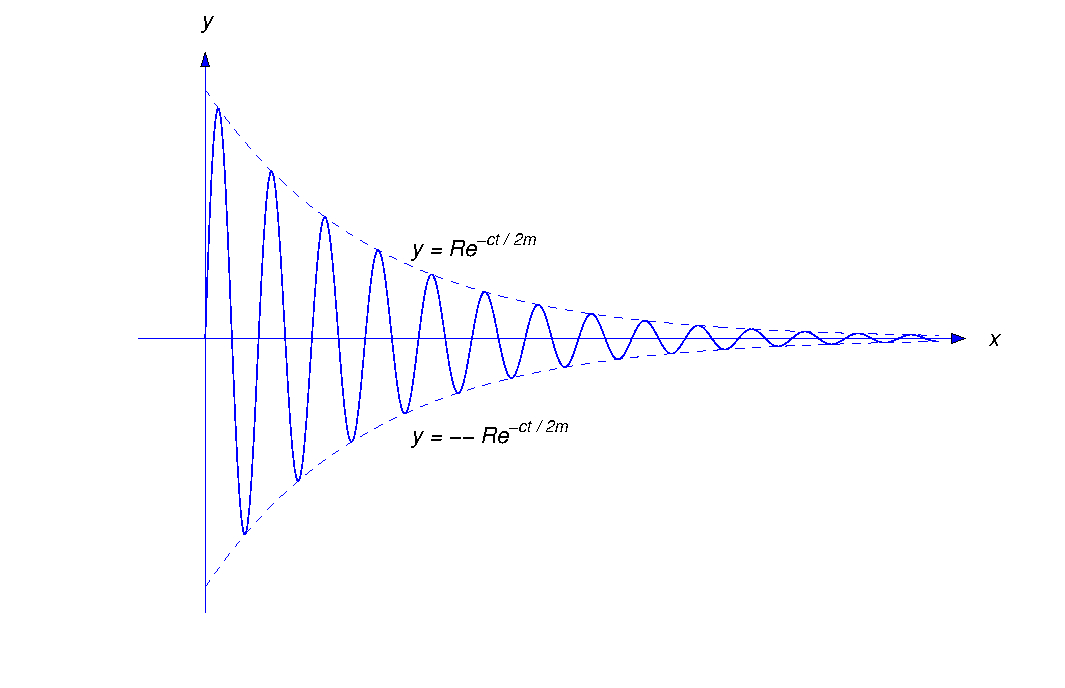
\includegraphics[height=1.5in]{fig060201.jpg}
\end{image}
 
As illustrated in that figure, the graph of $y$
oscillates between the dashed exponential curves $y=\pm Re^{-ct/2m}$.
 
\subsection*{Overdamped Motion}
 
We say the motion is \textit{overdamped} if $c>\sqrt{4mk}$. In this
case the zeros $r_1$ and $r_2$ of the characteristic polynomial are
real, with $r_1<r_2<0$ (see \eqref{eq:6.2.2}), and the general solution of
\eqref{eq:6.2.1} is
$$
y=c_1e^{r_1t}+c_2e^{r_2t}.
$$
Again $\lim_{t\rightarrow\infty}y(t)=0$ as in the
underdamped case, but the motion isn't  oscillatory, since $y$ can't
equal zero for more than one value of $t$ unless $c_1=c_2=0$.
%(Exercise~\ref{exer:6.2.23}.)
 
\subsection*{Critically Damped Motion}
 
We say the motion is \textit{critically damped} if $c=\sqrt{4mk}$. In
this case $r_1=r_2=-c/2m$ and the general solution of \eqref{eq:6.2.1} is
$$
y=e^{-ct/2m}(c_1+c_2t).
$$
 
Again $\lim_{t\rightarrow\infty}y(t)=0$ and the motion is nonoscillatory,
since $y$ can't equal zero for more than one value of $t$ unless
$c_1=c_2=0$. %(Exercise~\ref{exer:6.2.22}).
 
\begin{example}\label{example:6.2.1}
Suppose a 64 lb weight stretches a spring 6 inches in equilibrium
and a dashpot provides a damping force of $c$ lb for each ft/sec of
velocity.
\begin{enumerate}
\item\label{item:6.2.1a} % (a)
 Write the equation of motion of the object and determine the value of
$c$ for which the motion is critically damped.
\item\label{item:6.2.1b} % (b)
 Find the displacement $y$ for $t>0$ if the motion is critically damped
and the initial conditions are $y(0)=1$ and $y'(0)=20$.
\item\label{item:6.2.1c} % (c)
 Find the displacement $y$ for $t>0$ if the motion is critically damped
and the initial conditions are $y(0)=1$ and $y'(0)=-20$.
\end{enumerate}
 
\begin{explanation}\ref{item:6.2.1a}  Here $m=2$ slugs and $k=64/.5=128$
lb/ft. Therefore the equation of motion  \eqref{eq:6.2.1} is
\begin{equation}\label{eq:6.2.4}
2y''+cy'+128y=0.
\end{equation}
The characteristic equation  is
$$
2r^2+cr+128=0,
$$
which has  roots
$$
r=\frac{-c\pm\sqrt{c^2-8\cdot128}}{4}.
$$
Therefore the damping is critical if
$$
c=\sqrt{8\cdot128}=32\mbox{ lb--sec/ft}.
$$
 
\ref{item:6.2.1b}
 Setting $c=32$ in  \eqref{eq:6.2.4} and cancelling the common factor $2$
yields
$$
y''+16y+64y=0.
$$
The characteristic equation  is
$$
r^2+16r+64y=(r+8)^2=0.
$$
Hence, the general solution is
\begin{equation}\label{eq:6.2.5}
y=e^{-8t}(c_1+c_2t).
\end{equation}
 Differentiating this yields
\begin{equation}\label{eq:6.2.6}
y'=-8y+c_2e^{-8t}.
\end{equation}
Imposing the initial conditions $y(0)=1$ and $y'(0)=20$ in the last
two equations shows that $1=c_1$ and $20=-8+c_2$. Hence, the solution
of the initial value problem is
$$
y=e^{-8t}(1+28t).
$$
Therefore the object approaches equilibrium from above as
$t\rightarrow\infty$. There's no oscillation.
 
\ref{item:6.2.1c}
Imposing the initial conditions $y(0)=1$ and $y'(0)=-20$ in
\eqref{eq:6.2.5} and \eqref{eq:6.2.6} yields $1=c_1$ and $-20=-8+c_2$. Hence,
the solution of this initial value problem is
$$
y=e^{-8t}(1-12t).
$$
Therefore the object moves downward through equilibrium just once,
and then approaches equilibrium from below as $t\rightarrow\infty$. Again,
there's no oscillation. The solutions of these two initial value
problems are graphed in the figure below.
 
\begin{image}
  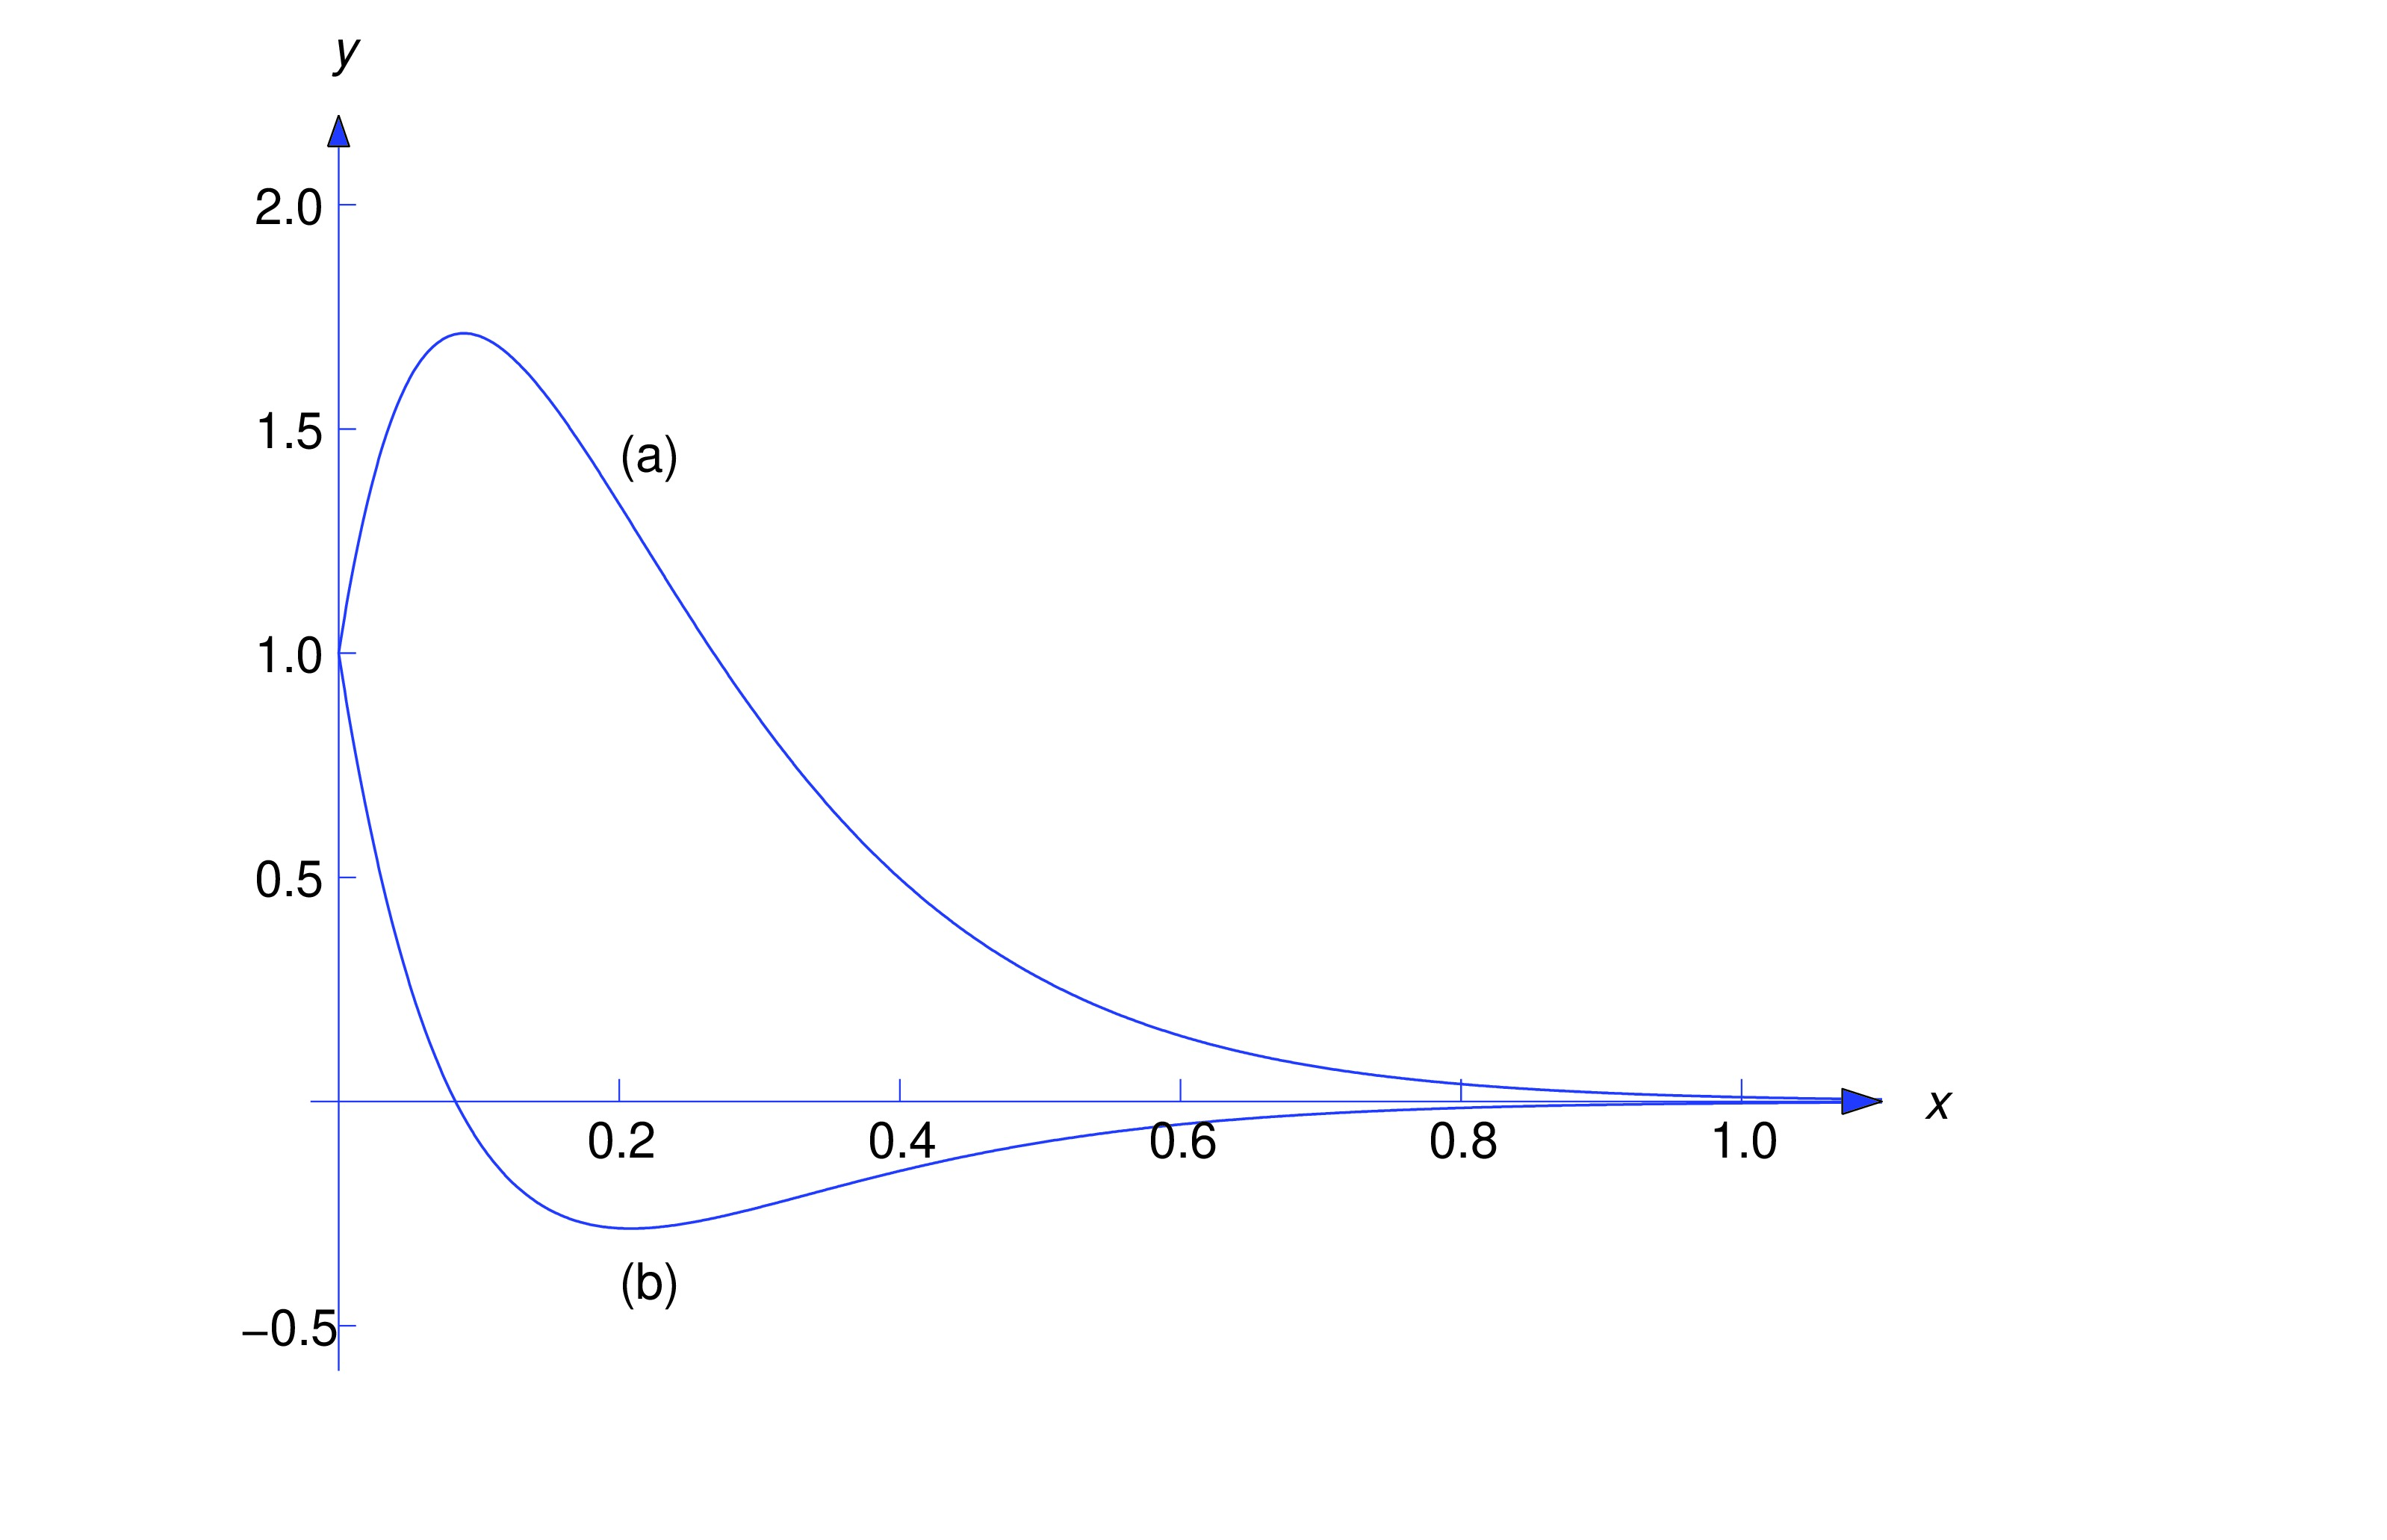
\includegraphics[height=1.5in]{fig060202.jpg}
\end{image}
 
\end{explanation}
\end{example}
 
\begin{example}
\label{example:6.2.2}
Find the displacement of the object in Example~\ref{example:6.2.1} if the
damping constant is $c=4$ lb--sec/ft and the initial conditions are
$y(0)=1.5$ ft and $y'(0)=-3$ ft/sec.
 
\begin{explanation}
With $c=4$, the equation of motion \eqref{eq:6.2.4} becomes
\begin{equation}\label{eq:6.2.7}
y''+2y'+64y=0
\end{equation}
after cancelling the common factor 2. The characteristic equation
$$
r^2+2r+64=0
$$
has complex conjugate roots
$$
r=\frac{-2\pm\sqrt{4-4\cdot64}}{2}=-1\pm3\sqrt7i.
$$
Therefore the motion is underdamped and the
general solution of  \eqref{eq:6.2.7} is
$$
y=e^{-t}(c_1\cos3\sqrt7t+c_2\sin3\sqrt7t).
$$
Differentiating this yields
$$
y'=-y+3\sqrt7e^{-t}(-c_1\sin3\sqrt7t+c_2\cos3\sqrt7t).
$$
Imposing the initial conditions $y(0)=1.5$ and $y'(0)=-3$ in the last
two equations yields $1.5=c_1$ and $-3=-1.5+3\sqrt7c_2$. Hence, the
solution of the initial value problem is
\begin{equation}\label{eq:6.2.8}
y=e^{-t}\bigg(\frac{3}{2}\cos3\sqrt7t-\frac{1}{2\sqrt7}
\sin3\sqrt7t\bigg).
\end{equation}
 The amplitude of the function in parentheses is
$$
 R=\sqrt{\bigg(\frac{3}{2}\bigg)^2+\bigg(\frac{1}{2\sqrt7}\bigg)^2}
=\sqrt{\frac{9}{4}+\frac{1}{4\cdot7}}
=\sqrt{\frac{64}{4\cdot7}}=\frac{4}{\sqrt7}.
$$
Therefore we can rewrite  \eqref{eq:6.2.8} as
$$
y=\frac{4}{\sqrt7}e^{-t}\cos(3\sqrt7t-\phi),
$$
 where
$$
\cos\phi=\frac{3}{2R}=\frac{3\sqrt{7}}{8}\quad\mbox{and}\quad\sin\phi=-\frac{1}{2\sqrt{7}R}=
-\frac{1}{8}.
$$
Therefore $\phi\cong-.125$  radians.
\end{explanation}
\end{example}
 
\begin{example}\label{example:6.2.3}
Let the damping constant in Example 1 be $c=40$ lb--sec/ft. Find the
displacement $y$ for $t>0$ if $y(0)=1$ and $y'(0)=1$.
 
\begin{explanation}
With $c=40$, the equation of motion \eqref{eq:6.2.4} reduces to
\begin{equation}\label{eq:6.2.9}
y''+20y'+64y=0
\end{equation}
 after cancelling the  common factor 2.
The characteristic equation
$$
r^2+20r+64=(r+16)(r+4)=0
$$
 has the roots $r_1=-4$ and $r_2=-16$.  Therefore the general
solution of  \eqref{eq:6.2.9} is
\begin{equation}\label{eq:6.2.10}
y=c_1e^{-4t}+c_2e^{-16t}.
\end{equation}
 Differentiating this yields
$$
y'=-4e^{-4t}-16c_2e^{-16t}.
$$
The last two equations and the initial conditions $y(0)=1$ and $y'(0)=1$
imply that
$$
\begin{array}{rlrl}
c_1&+&c_2&=1\\
-4c_1&-&16c_2&=1.
\end{array}
$$
 The solution of this system is $c_1=17/12$, $c_2=-5/12$.
Substituting these into  \eqref{eq:6.2.10} yields
$$
y=\frac{17}{12}e^{-4t}-\frac{5}{12}e^{-16t}
$$
as the solution of the given initial value problem.
 
\begin{image}
  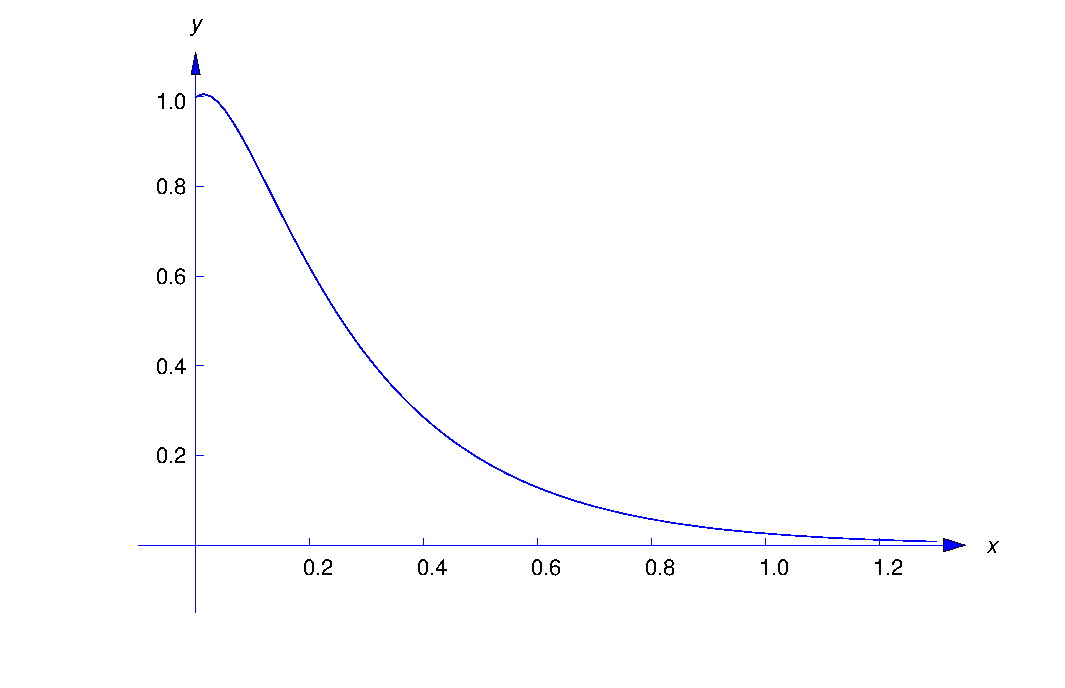
\includegraphics[height=1.5in]{fig060203.jpg}
\end{image}
 
 
\end{explanation}
\end{example}
 
\subsection{Forced Vibrations With Damping}
 
Now we consider the motion of an object in a spring-mass system with
damping, under the influence of a periodic forcing function
$F(t)=F_0\cos\omega t$, so that the equation of motion is
\begin{equation}\label{eq:6.2.11}
my''+cy'+ky=F_0\cos\omega t.
\end{equation}
In \href{https://ximera.osu.edu/ode/main/springProblemsI/springProblemsI}{Trench 6.1} we considered this equation with $c=0$ and
found that the resulting displacement $y$ assumed arbitrarily large
values in the case of resonance   (that is, when
$\omega=\omega_0=\sqrt{k/m}$). Here we'll see that in the presence
of damping the displacement remains bounded for all $t$, and the
initial conditions have little effect on the motion as $t\rightarrow\infty$.
In fact, we'll see that for large $t$ the displacement is closely
approximated by a function of the form
\begin{equation}\label{eq:6.2.12}
y=R\cos(\omega t-\phi),
\end{equation}
where the amplitude $R$ depends upon $m$, $c$, $k$, $F_0$, and
$\omega$. We're interested in the following question:
 
\begin{question}Assuming that $m$, $c$, $k$, and $F_0$ are
held constant, what value of $\omega$ produces the largest amplitude
$R$ in \eqref{eq:6.2.12}, and what is this largest amplitude?
\end{question}
 
To answer this question, we must solve \eqref{eq:6.2.11} and determine $R$ in
terms of $F_0,\omega_0,\omega$, and $c$. We can obtain a particular
solution of \eqref{eq:6.2.11} by the method of undetermined coefficients.
Since $\cos\omega t$ does not satisfy the complementary equation
$$
my''+cy'+ky=0,
$$
we can obtain a particular solution of \eqref{eq:6.2.11} in the form
\begin{equation}\label{eq:6.2.13}
y_p=A\cos\omega t+B\sin\omega t.
\end{equation}
Differentiating this yields
$$
y_p'=\quad\omega (-A\sin\omega t+B\cos\omega t)
$$
and
$$
y_p''=-\omega^2(A\cos\omega t+B\sin\omega t).
$$
 From the last three equations,
$$
my''_p+cy'_p+ky_p=(-m\omega^2A+c\omega B+kA)\cos\omega t+
(-m\omega^2 B-c\omega A+kB)\sin\omega t,
$$
so $y_p$ satisfies  \eqref{eq:6.2.11}  if
$$
\begin{array}{lll}
(k-m\omega^2) A+\quad c\omega B &=&F_0\\
-c\omega A\quad+(k-m\omega^2)B&=&0.
\end{array}
$$
 
 
 Solving  for $A$ and $B$
and substituting the results into  \eqref{eq:6.2.13} yields
$$
y_p=\frac{F_0}{(k-m\omega^2)^2+c^2\omega^2}
\left[(k-m\omega^2)\cos\omega t+c\omega\sin\omega t\right],
$$
which can be written in amplitude--phase form  as
\begin{equation}\label{eq:6.2.14} %\springsteady
y_p=\frac{F_0}{\sqrt{(k-m\omega^2)^2+c^2\omega^2}}
\cos(\omega t-\phi),
\end{equation}
where
\begin{equation}\label{eq:6.2.15}
\cos\phi=\frac{k-m\omega^2}{\sqrt
{(k-m\omega^2)^2+c^2\omega^2}}\quad\mbox{and}\quad
\sin\phi=\frac{c\omega}{\sqrt{(k-m\omega^2)^2+c^2\omega^2}}.
\end{equation}
 
  To compare this with the undamped forced vibration
that we considered in the previous module, it's useful to write
\begin{equation}\label{eq:6.2.16}
k-m\omega^2=m\bigg(\frac{k}{m}-\omega^2\bigg)=
m(\omega_0^2-\omega^2),
\end{equation}
 where $\omega_0=\sqrt{k/m}$ is the natural
angular frequency of the undamped simple harmonic motion of an
object with mass $m$ on a spring with constant $k$.
Substituting  \eqref{eq:6.2.16} into  \eqref{eq:6.2.14} yields
\begin{equation}\label{eq:6.2.17}
y_p=\frac{F_0}{\sqrt{m^2(\omega^2_0-\omega^2)^2+
c^2\omega^2}}\cos(\omega t-\phi).
\end{equation}
 
The solution of an initial value problem
$$
my''+cy'+ky=F_0\cos\omega t, \quad  y(0)=y_0,\quad y'(0)=v_0,
$$
is of the form $y=y_c+y_p$,
where  $y_c$ has one of the three forms
\begin{eqnarray*}
y_c&=&e^{-ct/2m}(c_1\cos\omega_1t+c_2\sin\omega_1t),\\
 y_c&=&e^{-ct/2m}(c_1+c_2t),\\
y_c&=&c_1e^{r_1t}+c_2e^{r_2t}\,(r_1,r_2<0).
\end{eqnarray*}
In all three cases $\lim_{t\rightarrow\infty} y_c(t)=0$ for any choice of
$c_1$ and $c_2$. For this reason we say that $y_c$ is the \textit{transient component} of the solution $y$. The behavior of $y$ for
large $t$ is determined by $y_p$, which we call the \textit{steady state
component} of $y$. Thus, for large $t$ the motion is like simple
harmonic motion at the frequency of the external force.
 
The amplitude of $y_p$ in \eqref{eq:6.2.17} is
\begin{equation}\label{eq:6.2.18}
R=\frac{F_0}{\sqrt{m^2(\omega^2_0-\omega^2)^2+c^2\omega^2}},
\end{equation}
which is finite for all $\omega$; that is, the presence of damping
precludes the phenomenon of resonance that we encountered in studying
undamped vibrations under a periodic forcing function. We'll now
find the value $\omega_{\max}$ of $\omega$ for which $R$ is maximized.
This is the value of $\omega$ for which the function
$$
\rho (\omega)=m^2(\omega^2_0-\omega^2)^2+c^2\omega^2
$$
in the denominator of  \eqref{eq:6.2.18} attains its minimum value.  By
rewriting this as
\begin{equation}\label{eq:6.2.19}
\rho (\omega)=m^2(\omega^4_0+\omega^4)+
 (c^2-2m^2\omega^2_0)\omega^2,
\end{equation}
 you can see that $\rho$ is a strictly
increasing function of $\omega^2$ if
$$
c\geq\sqrt{2m^2\omega^2_0}=\sqrt{2mk}.
$$
(Recall that $\omega^2_0=k/m$). Therefore $\omega_{\max}=0$ if this
inequality holds. From \eqref{eq:6.2.15}, you can see that $\phi=0$ if
$\omega=0$. In this case, \eqref{eq:6.2.14} reduces to
$$
y_p=\frac{F_0}{\sqrt{m^2\omega^4_0}}=\frac{F_0}{k},
$$
which is consistent with Hooke's law: if the mass is subjected to a
constant force $F_0$,  its displacement should approach a constant
$y_p$ such that $ky_p=F_0$. Now suppose   $c<\sqrt{2mk}$. Then,
from \eqref{eq:6.2.19},
$$
\rho'(\omega)=2\omega(2m^2\omega^2+c^2-2m^2\omega^2_0),
$$
and $\omega_{\max}$ is the value of $\omega$ for which the
expression in parentheses equals zero; that is,
$$
\omega_{\max}=\sqrt{\omega^2_0-\frac{c^2}{2m^2}}
=\sqrt{\frac{k}{m}\left(1-\frac{c^2}{2km}\right)}.
$$
(To see that $\rho(\omega_{\max})$ is the minimum value of
$\rho(\omega)$, note that $\rho'(\omega)<0$ if $\omega
<\omega_{\max}$ and $\rho'(\omega)>0$ if $\omega>\omega_{\max}$.)
Substituting $\omega=\omega_{\max}$ in \eqref{eq:6.2.18} and simplifying
shows that the maximum amplitude $R_{\max}$ is
$$
R_{\max}=\frac{2mF_0}{c\sqrt{4mk-c^2}}\quad \mbox{if}\quad c<
\sqrt{2mk}.
$$
We summarize our results  as follows.
 
 
\begin{theorem} \label{thmtype:6.2.1}
 Suppose we consider the amplitude $R$ of the steady state
component of the solution of
$$
my''+cy'+ky=F_0\cos\omega t
$$
as a function of $\omega$.
\begin{enumerate}
    \item
 If $c\geq\sqrt{2mk}$,  the maximum amplitude is
 $R_{\max}=F_0/k$ and it's attained when $\omega=
\omega_{\max}=0$.
\item
If $c<\sqrt{2mk}$, the maximum amplitude is
\begin{equation}\label{eq:6.2.20}
R_{\max}=\frac{2m F_0}{c\sqrt{4mk-c^2}},
\end{equation}
and it's attained when
\begin{equation}\label{eq:6.2.21}
\omega=\omega_{\max}=\sqrt{\frac{k}{m}\left(1-\frac{c^2}{2km}\right)}.
\end{equation}
\end{enumerate}
\end{theorem}
Note that $R_{\max}$ and $\omega_{\max}$ are continuous functions
of $c$, for $c\geq0$, since  \eqref{eq:6.2.20} and  \eqref{eq:6.2.21} reduce
to $R_{\max}=F_0/k$ and $\omega_{\max}=0$ if $c=\sqrt{2km}$.
 
 
\section*{Text Source}
Trench, William F., "Elementary Differential Equations" (2013). Faculty Authored and Edited Books \& CDs. 8. (CC-BY-NC-SA)
 
\href{https://digitalcommons.trinity.edu/mono/8/}{https://digitalcommons.trinity.edu/mono/8/}
 
\end{document}